\section{Referencia de la Clase Factura}
\label{classFactura}\index{Factura@{Factura}}
Administra los datos de una factura a cliente.  


{\tt \#include $<$factura.h$>$}

Diagrama de herencias de Factura\begin{figure}[H]
\begin{center}
\leavevmode
\includegraphics[width=101pt]{classFactura__inherit__graph}
\end{center}
\end{figure}
Diagrama de colaboraci\'{o}n para Factura:\begin{figure}[H]
\begin{center}
\leavevmode
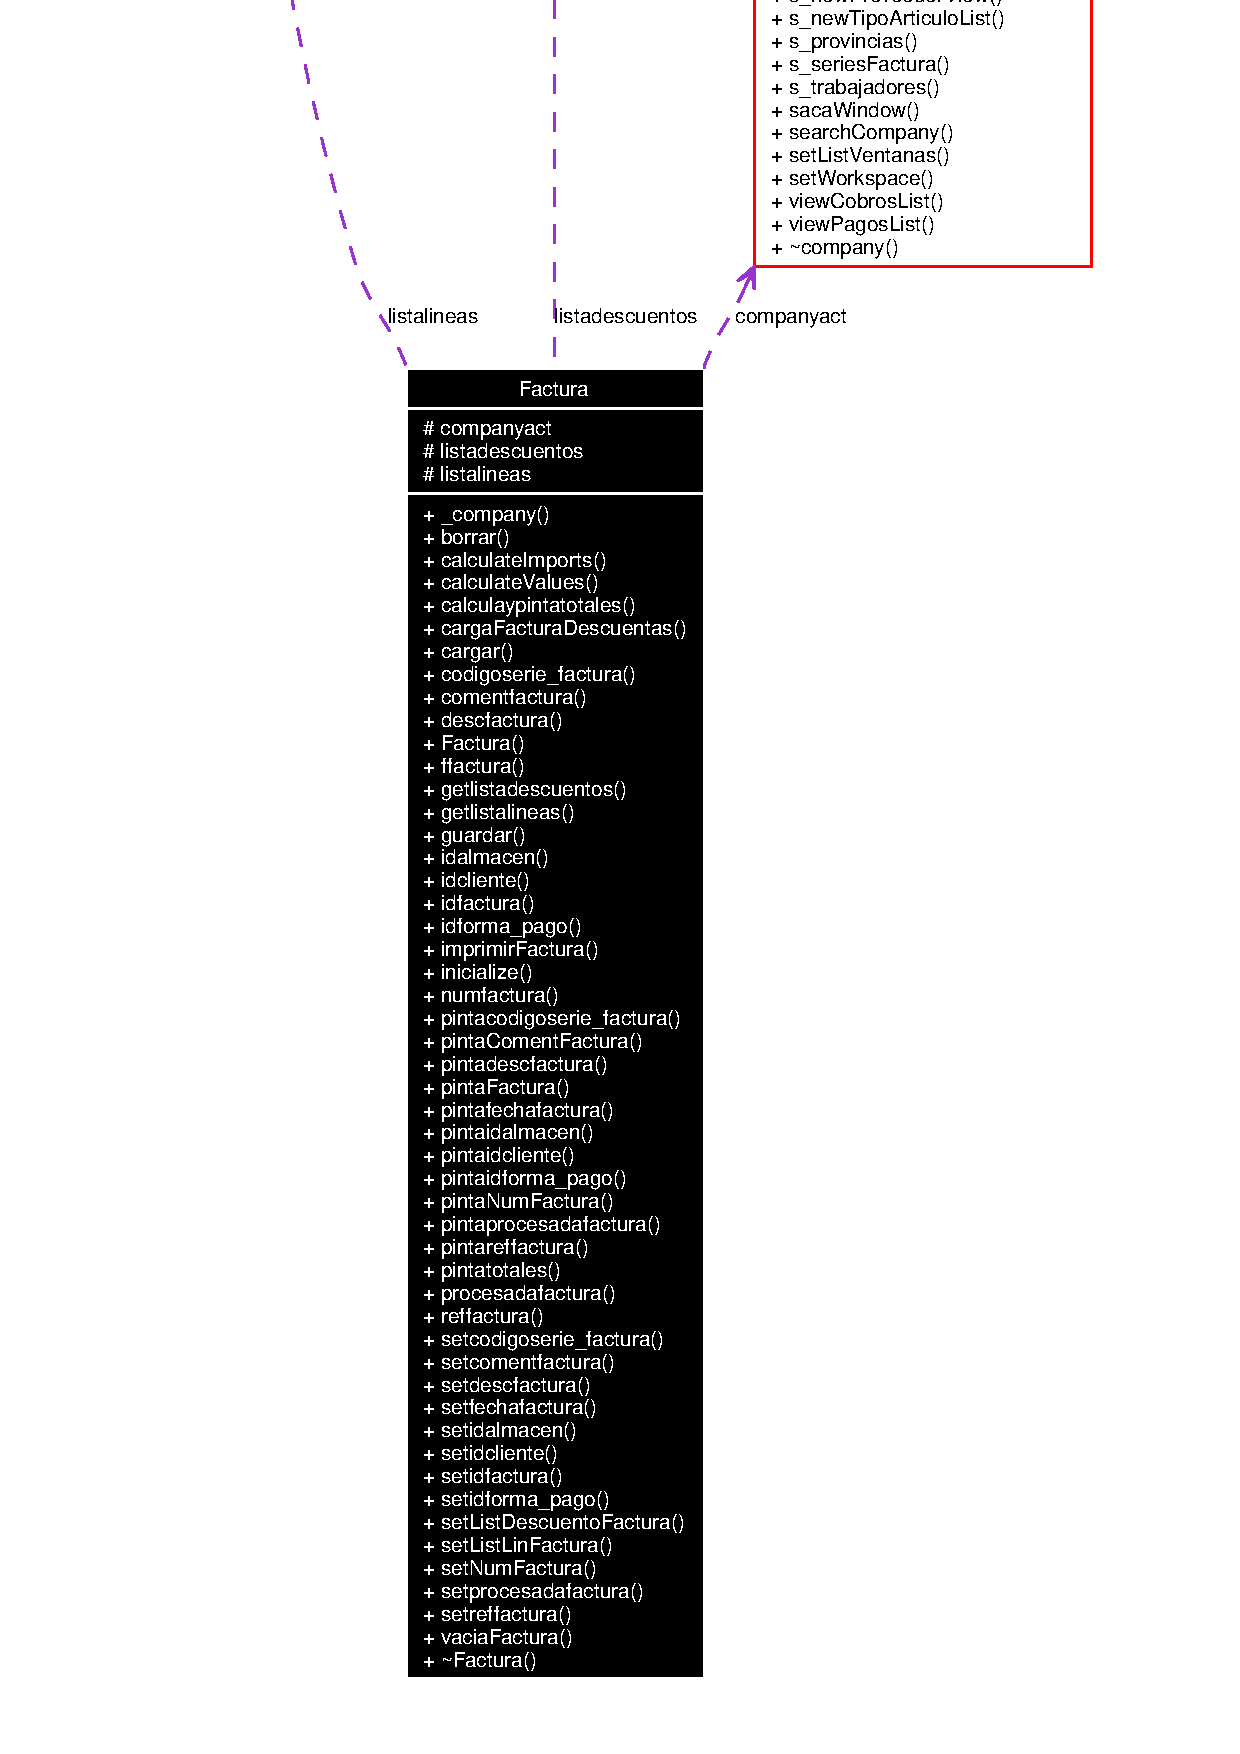
\includegraphics[width=262pt]{classFactura__coll__graph}
\end{center}
\end{figure}
\subsection*{M\'{e}todos p\'{u}blicos}
\begin{CompactItemize}
\item 
{\bf company} $\ast$ {\bf \_\-company} ()\label{classFactura_a0}

\item 
virtual int {\bf borrar} ()\label{classFactura_a1}

\item 
virtual void {\bf calculate\-Imports} ()\label{classFactura_a2}

\item 
virtual QString {\bf calculate\-Values} ()\label{classFactura_a3}

\item 
virtual void {\bf calculaypintatotales} ()
\item 
virtual void {\bf carga\-Factura\-Descuentas} (QString)\label{classFactura_a5}

\item 
virtual int {\bf cargar} (QString)\label{classFactura_a6}

\begin{CompactList}\small\item\em Esta funcion carga un factura. \item\end{CompactList}\item 
QString {\bf codigoserie\_\-factura} ()\label{classFactura_a7}

\item 
QString {\bf comentfactura} ()\label{classFactura_a8}

\item 
QString {\bf descfactura} ()\label{classFactura_a9}

\item 
{\bf Factura} ({\bf company} $\ast$)\label{classFactura_a10}

\item 
QString {\bf ffactura} ()\label{classFactura_a11}

\item 
{\bf List\-Descuento\-Factura\-View} $\ast$ {\bf getlistadescuentos} ()\label{classFactura_a12}

\item 
{\bf List\-Lin\-Factura\-View} $\ast$ {\bf getlistalineas} ()\label{classFactura_a13}

\item 
virtual int {\bf guardar} ()
\item 
QString {\bf idalmacen} ()\label{classFactura_a15}

\item 
QString {\bf idcliente} ()\label{classFactura_a16}

\item 
QString {\bf idfactura} ()\label{classFactura_a17}

\item 
QString {\bf idforma\_\-pago} ()\label{classFactura_a18}

\item 
virtual void {\bf imprimir\-Factura} ()
\item 
virtual void {\bf inicialize} ()\label{classFactura_a20}

\item 
QString {\bf numfactura} ()\label{classFactura_a21}

\item 
virtual void {\bf pintacodigoserie\_\-factura} (QString)\label{classFactura_a22}

\item 
virtual void {\bf pinta\-Coment\-Factura} (QString)\label{classFactura_a23}

\item 
virtual void {\bf pintadescfactura} (QString)\label{classFactura_a24}

\item 
void {\bf pinta\-Factura} ()
\item 
virtual void {\bf pintafechafactura} (QString)\label{classFactura_a26}

\item 
virtual void {\bf pintaidalmacen} (QString)\label{classFactura_a27}

\item 
virtual void {\bf pintaidcliente} (QString)\label{classFactura_a28}

\item 
virtual void {\bf pintaidforma\_\-pago} (QString)\label{classFactura_a29}

\item 
virtual void {\bf pinta\-Num\-Factura} (QString)\label{classFactura_a30}

\item 
virtual void {\bf pintaprocesadafactura} (QString)\label{classFactura_a31}

\item 
virtual void {\bf pintareffactura} (QString)\label{classFactura_a32}

\item 
virtual void {\bf pintatotales} (Fixed, Fixed, Fixed, Fixed)\label{classFactura_a33}

\item 
QString {\bf procesadafactura} ()\label{classFactura_a34}

\item 
QString {\bf reffactura} ()\label{classFactura_a35}

\item 
void {\bf setcodigoserie\_\-factura} (QString val)\label{classFactura_a36}

\item 
void {\bf setcomentfactura} (QString val)\label{classFactura_a37}

\item 
void {\bf setdescfactura} (QString val)\label{classFactura_a38}

\item 
void {\bf setfechafactura} (QString val)\label{classFactura_a39}

\item 
void {\bf setidalmacen} (QString val)\label{classFactura_a40}

\item 
void {\bf setidcliente} (QString val)\label{classFactura_a41}

\item 
void {\bf setidfactura} (QString val)\label{classFactura_a42}

\item 
void {\bf setidforma\_\-pago} (QString val)\label{classFactura_a43}

\item 
void {\bf set\-List\-Descuento\-Factura} ({\bf List\-Descuento\-Factura\-View} $\ast$a)\label{classFactura_a44}

\item 
void {\bf set\-List\-Lin\-Factura} ({\bf List\-Lin\-Factura\-View} $\ast$a)
\item 
void {\bf set\-Num\-Factura} (QString val)\label{classFactura_a46}

\item 
void {\bf setprocesadafactura} (QString val)\label{classFactura_a47}

\item 
void {\bf setreffactura} (QString val)\label{classFactura_a48}

\item 
void {\bf vacia\-Factura} ()\label{classFactura_a49}

\end{CompactItemize}
\subsection*{Atributos protegidos}
\begin{CompactItemize}
\item 
{\bf company} $\ast$ {\bf companyact}\label{classFactura_p0}

\item 
{\bf List\-Descuento\-Factura\-View} $\ast$ {\bf listadescuentos}\label{classFactura_p1}

\item 
{\bf List\-Lin\-Factura\-View} $\ast$ {\bf listalineas}\label{classFactura_p2}

\end{CompactItemize}


\subsection{Descripci\'{o}n detallada}
Administra los datos de una factura a cliente. 



\subsection{Documentaci\'{o}n de las funciones miembro}
\index{Factura@{Factura}!calculaypintatotales@{calculaypintatotales}}
\index{calculaypintatotales@{calculaypintatotales}!Factura@{Factura}}
\subsubsection{\setlength{\rightskip}{0pt plus 5cm}void Factura::calculaypintatotales ()\hspace{0.3cm}{\tt  [virtual]}}\label{classFactura_a4}


Impresion de los contenidos.

Impresion de los descuentos. \index{Factura@{Factura}!guardar@{guardar}}
\index{guardar@{guardar}!Factura@{Factura}}
\subsubsection{\setlength{\rightskip}{0pt plus 5cm}int Factura::guardar ()\hspace{0.3cm}{\tt  [virtual]}}\label{classFactura_a14}


Calculamos el proximo numero de factura para poder insertarlo en caso de que este sea nulo. 

Reimplementado en {\bf Factura\-View} {\rm (p.\,\pageref{classFacturaView_a3})}.\index{Factura@{Factura}!imprimirFactura@{imprimirFactura}}
\index{imprimirFactura@{imprimirFactura}!Factura@{Factura}}
\subsubsection{\setlength{\rightskip}{0pt plus 5cm}void Factura::imprimir\-Factura ()\hspace{0.3cm}{\tt  [virtual]}}\label{classFactura_a19}


Hacemos el lanzamiento de plugins para este caso.

Copiamos el archivo.

Copiamos el logo.

Linea de totales del presupuesto.

Impresion de la tabla de contenidos.

Impresion de los descuentos.

Impresion de los totales.

Rellena el primer tr de titulares.

Rellena el segundo tr de cantidades. \index{Factura@{Factura}!pintaFactura@{pintaFactura}}
\index{pintaFactura@{pintaFactura}!Factura@{Factura}}
\subsubsection{\setlength{\rightskip}{0pt plus 5cm}void Factura::pinta\-Factura ()}\label{classFactura_a25}


Pinta el subformulario de detalle del factura. \index{Factura@{Factura}!setListLinFactura@{setListLinFactura}}
\index{setListLinFactura@{setListLinFactura}!Factura@{Factura}}
\subsubsection{\setlength{\rightskip}{0pt plus 5cm}void Factura::set\-List\-Lin\-Factura ({\bf List\-Lin\-Factura\-View} $\ast$ {\em a})\hspace{0.3cm}{\tt  [inline]}}\label{classFactura_a45}


Establece cu\'{a}l es la lista subformulario del presupuesto. Normalmente para apuntar listlinpresupuestoview. 

La documentaci\'{o}n para esta clase fu\'{e} generada a partir de los siguientes archivos:\begin{CompactItemize}
\item 
factura.h\item 
factura.cpp\end{CompactItemize}
